\documentclass[journal]{IEEEtran}
\usepackage{cite}
\usepackage[dvips]{graphicx}
\usepackage{hyperref}

\begin{document}
\title{Optical phase characterization of integrated photonic devices}
\author{J.~Matres,~G.~C.~Ballesteros,~S.~Mas,~A.~Brimont,~P.~Sanchis,~J.~Mart\'i~and~C.~J.~Oton}
%\markboth{Journal of Lightwave Technology}%
%{Shell \MakeLowercase{\textit{J. Matres et al.}}: Optical phase characterization of integrated photonic devices}

\maketitle


\begin{abstract}
We propose a relatively simple experimental setup capable of accurately characterizing the optical phase response of an integrated photonic circuit. The setup is based on a phase-noise reduction scheme using an external heterodyne Mazch-Zehnder interferometer. In particular, we characterize the phase response of different silicon photonic components: undercoupled and overcoupled ring resonators, and a slow light corrugated waveguide.
\end{abstract}

\section{Introduction}
\noindent Standardization and technological advances have remarkably developed integrated optics in the last years.
With hundreds of components on a small footprint, one can build extremely complex systems at a very low cost per device.
In designing any system, the phase response of each component is a key parameter.
However, phase noise prevents simple interferometric measurements using, for example, an external Mach-Zehnder interferometer (MZI).


\emph{Optical vector network analyzers} (OVNA) are commercial devices sensitive to phase~\cite{Vanwiggeren2003, Gifford2005}.
They employ specific techniques to alleviate phase noise problems in their measurement, requiring very fast laser tuning speeds (higher than 100~nm/s) and complex synchronous receiving schemes.
Fast laser sweeping reduces phase noise, as thermally-induced noise usually has a 1/f spectral dependence.


In this work, we present an accurate and continuous phase response using an ordinary laser with a tuning speed below 1~nm/s.
We cancel the phase noise employing a counter-propagating reference beam at fixed wavelength.
In Ref.~\cite{Mas2012} we applied the same idea to characterize chromatic dispersion in waveguides with different geometries.
In this paper we characterize the phase response of different building blocks, in particular, a silicon micro-ring resonator and corrugated waveguide.
In the former, we distinguish undercoupling from overcoupling conditions and extract the parameters of the ring.
In the latter, we plot the group index of the corrugation from a single segment of waveguide without the need of integrated MZIs and fringe spacing calculations.


\section{Experimental setup}
The experimental setup is a fiber-based MZI, where acousto-optic modulators (AOM) act as frequency shifters (Fig.~\ref{fig:dispersionSetup}).
Each branch applies a slightly different frequency shift (40~kHz in our experiment) and the lock-in amplifier measures the 40~kHz beating pattern.
The phase of these beatings with respect to the RF generators provides the phase of the system, but they are affected by thermal phase noise as high as several radians per second. 
This noise would make unfeasible a phase characterization using a laser with few nm/s tuning speed.
To cancel the phase noise, we introduce from the opposite end a reference counter-propagating beam at a fixed wavelength.
This signal produces another beating pattern used as a reference for the lock-in amplifier.
As thermal fluctuations equally affect both beams, they cancel out, measuring only the wavelength-dependent phase variations.



\begin{figure}[htb]
	\centering
	\includegraphics[width=3.5in]{dispersion5}
	\caption{The lock-in monitors the 40~KHz-beatings using a counter-propagating beam as a reference signal to compensate thermal fluctuations.}
	\label{fig:dispersionSetup}
\end{figure}



To balance the interferometer for different device lengths there is an optical delay line in the branch without sample.
Before each sweep is launched, the MZI must be balanced in order to avoid too steep slopes in the $\omega$ phase dependence.
In addition, it is convenient to set the wavelength of the counter-propagating reference beam, $\omega_0$, approximately in the middle of the sweep in order to get small phase noise.
If the building block to characterize is in series with other elements, (couplers, connecting waveguides, tapers, etc.) the measurement requires a reference sample with the same elements, but without the component under test (e.g. the corrugated waveguide).
The reference sweep provides the system response, which must be subtracted from the measurement with the component under test. 
Mathematically, the phase dependence obtained with the lock-in, after subtracting the system response, becomes:


\begin{equation}
  \phi(\omega)= \beta_c L_c - \beta_{air} \Delta L_{air} =\phi_{c}(\omega)-\frac{\omega\Delta L_{air}}{c}
  \label{eq:response}
\end{equation}

where $\phi$ is the measured phase, $\phi_{c}$ the phase introduced by the component under test, $\Delta L_{air}$ the extra length introduced in the optical delay line to balance the MZI with respect to the reference measurement, $\beta_c$ and $\beta_{air}$ the propagation constants of the component and of air respectively, and $c$ the speed of light in vacuum.
In Ref.~\cite{Mas2012} we demonstrated that if the component under test has a length $L_{c}$, then the the group index of the component is:

\begin{equation}
  n_{g} = \frac{\Delta L_{air}}{L_{c}}
  \label{eq:group_index_pathBalancing}
\end{equation}

Minimizing the phase versus wavelength slope balances the MZI.
A slope equal to zero at a certain wavelength corresponds to perfect balancing, so one can extract the group index of the component under test.
Finally, from the group index slope variation we extract its wavelength dependence (Section \ref{sec:corrWaveguides}).
It is worth mentioning that the lock-in simultaneously characterizes phase and amplitude in one single sweep.
Moreover, noise due to gradual slight misalignment cancels out normalizing with the amplitude of the reference signal.

\section{Experiment}
Samples were fabricated using the EPIXFAB platform, processed from 220~nm Si thickness SOI wafers, patterned with deep-UV lithography and covered with silica after the etching process.
They included 20~$\mu$m radius ring resonators and a corrugated waveguide.
In both cases we coupled transverse-electric (TE) light using grating couplers.

\begin{figure}[htb]
    \centering
    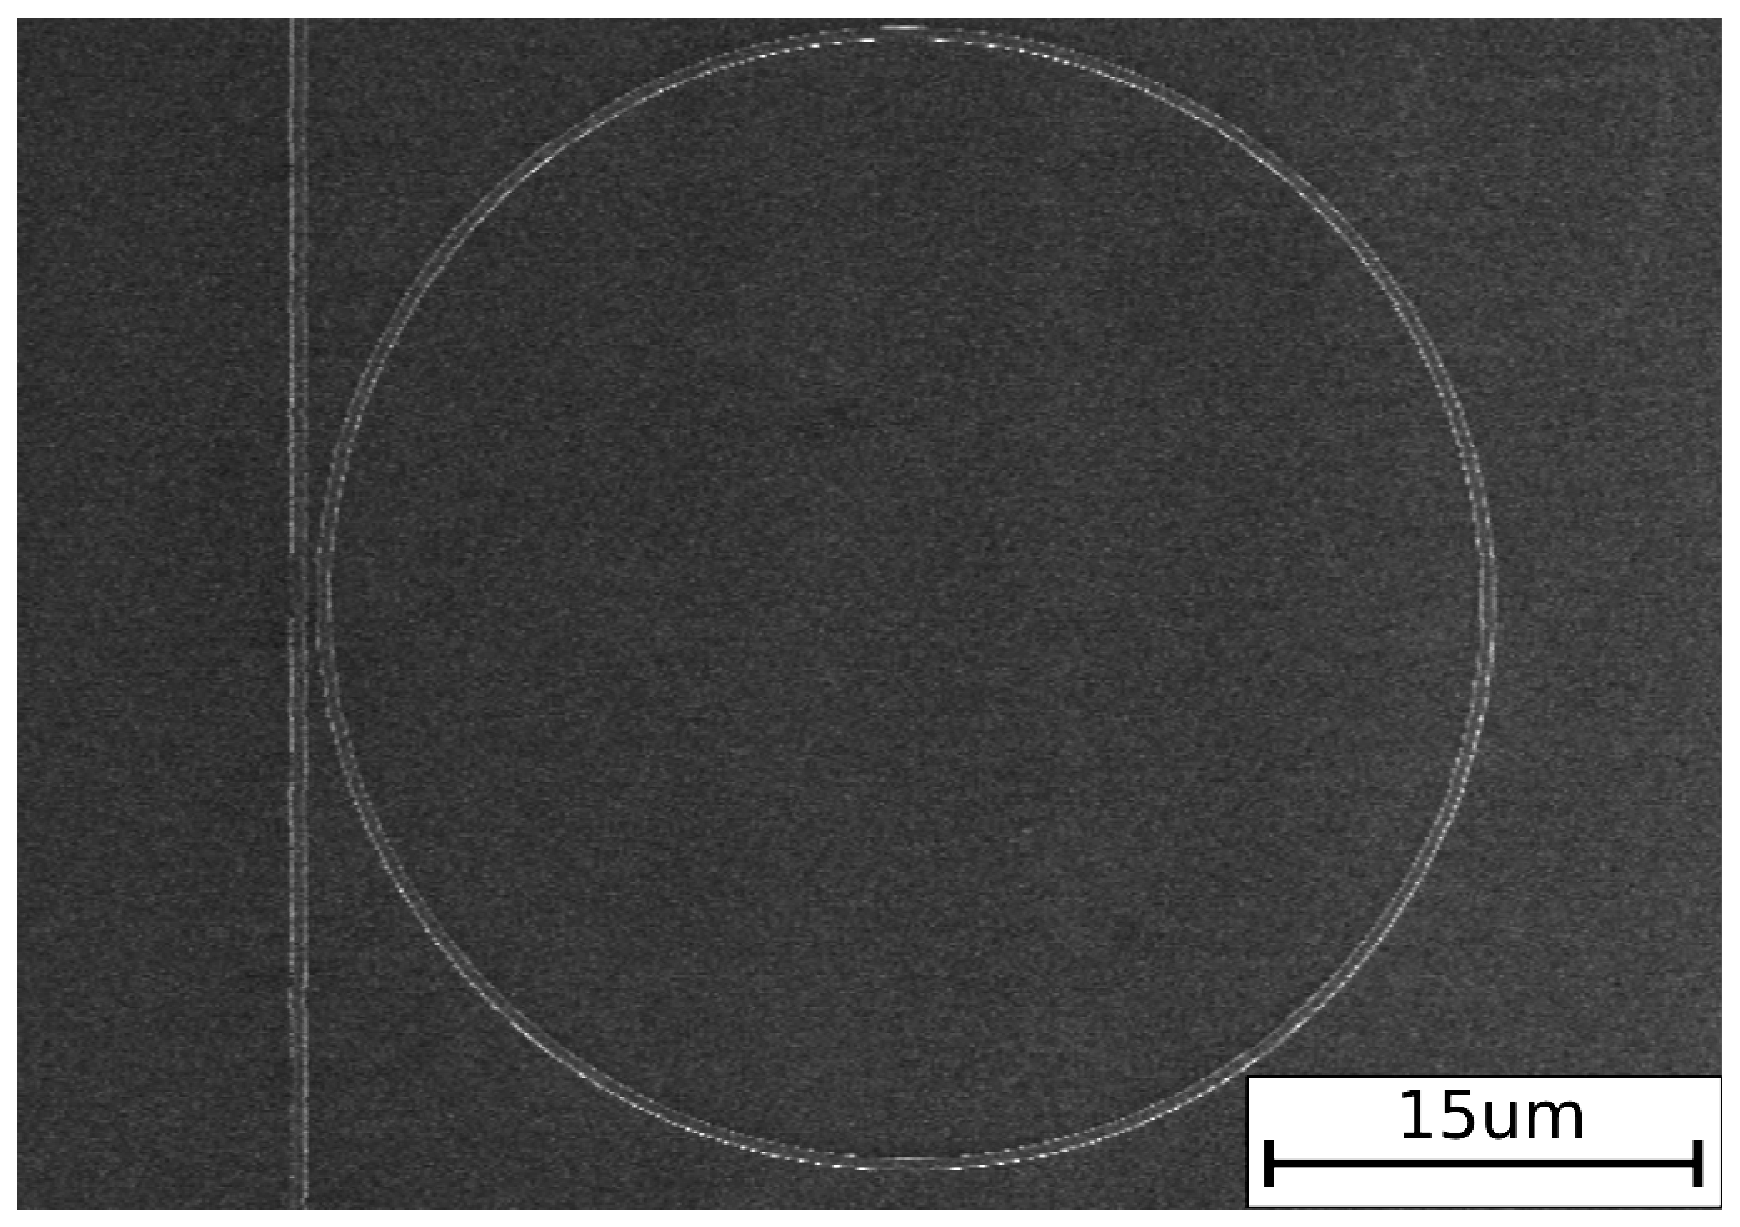
\includegraphics[width=2.5in]{ringTEscale2}
    \caption{Ring resonators are very useful components for filtering, multiplexing, switching and modulating.}
    \label{fig:semRingPaperRings}
\end{figure}


\begin{figure}[htb]
	\centering
	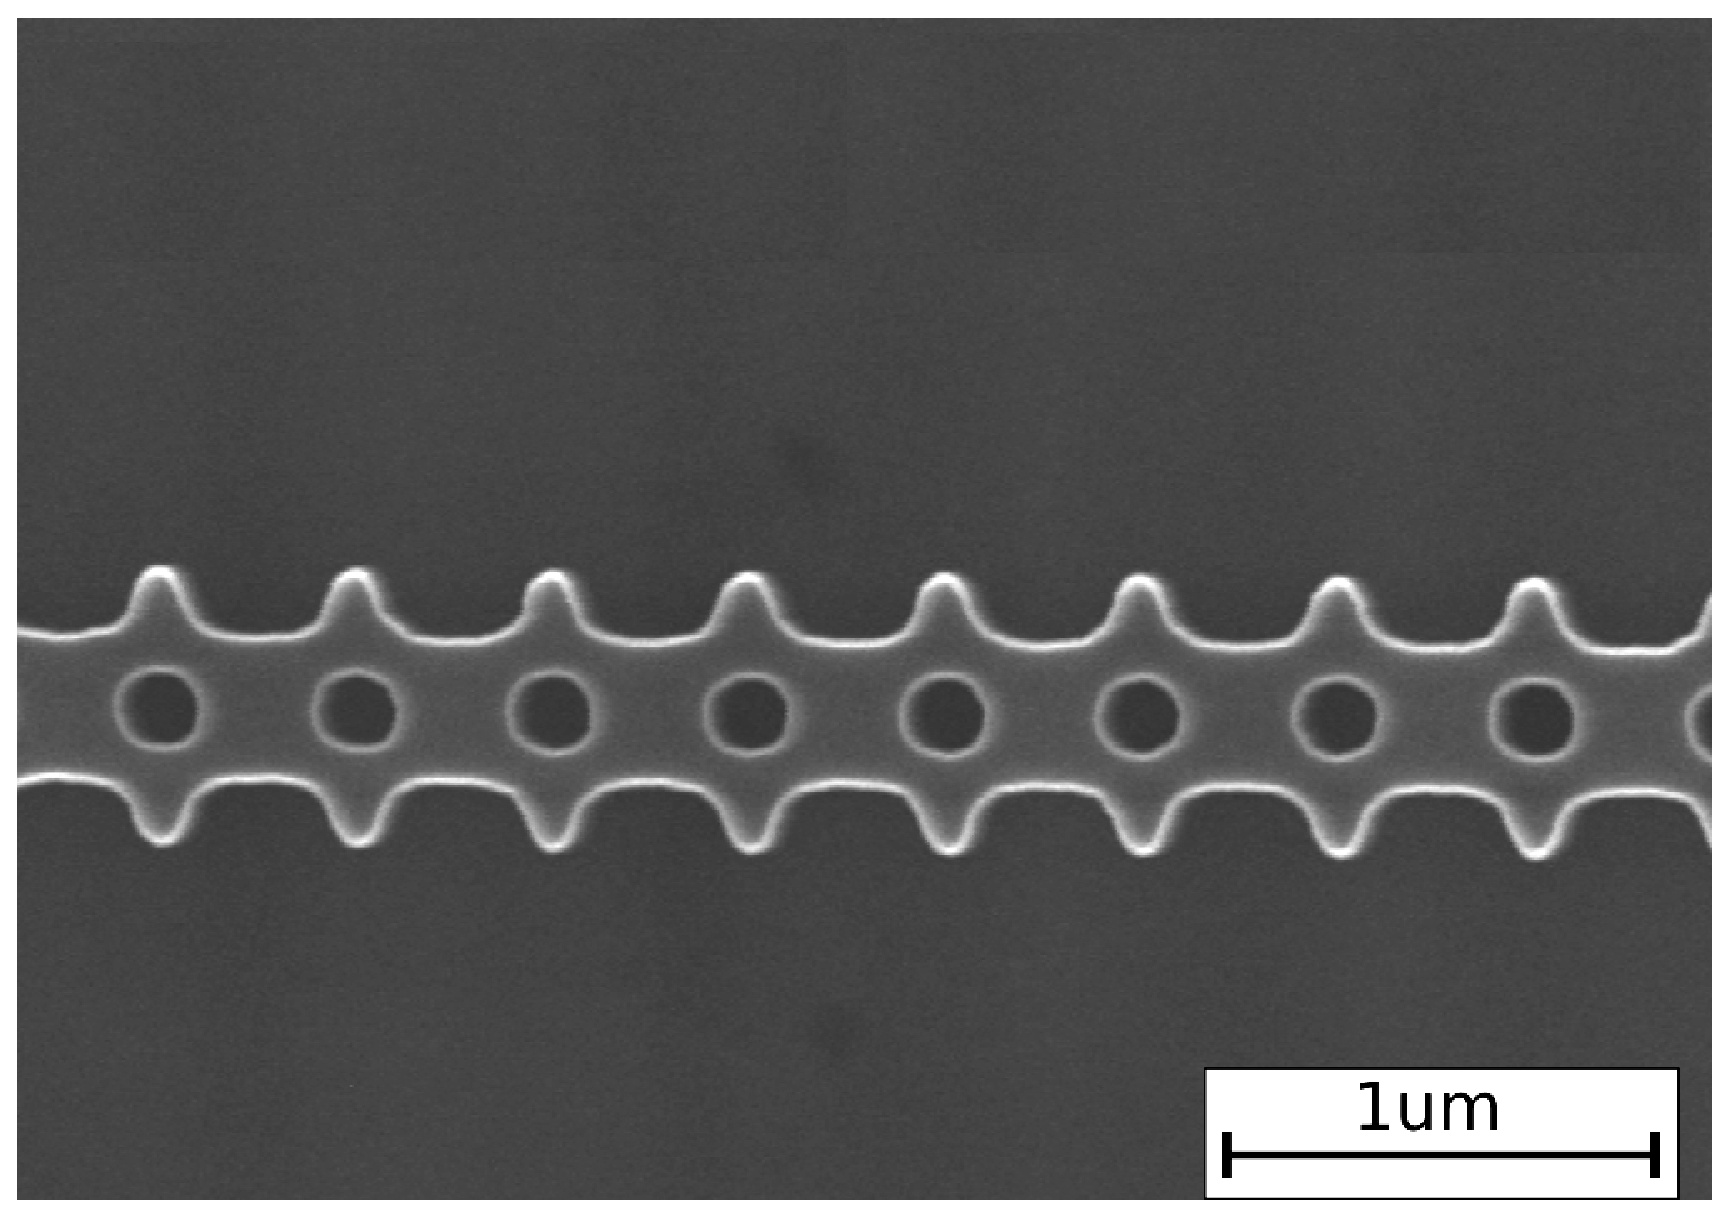
\includegraphics[width=2.5in]{corrTEscale}	
	\caption{Corrugated waveguides had a broadband flattened group index profile (from 1560 to 1610~nm), achievable by patterning circular holes onto the wide section of the waveguide as in~\cite{Brimont2010}.}
	\label{fig:sem}
 \end{figure} 


\subsection{Ring resonators parameter extraction}
\label{sec:ringResonators}

The most important parameters of rings resonators are the free spectral range (FSR), the extinction ratio (ER), and the width of the resonance (FWHM). These parameters depend not only in design but also manufacturing tolerances~\cite{Bogaerts:12}.

\begin{equation}
	FSR=\frac{\lambda_{res}^2}{n_gL}
	\label{eq:FSRanillo}
\end{equation} 

where $n_g$ is the group index and L is the round trip length.

The transmission equation of a ring can be easily obtained~\cite{McKinnon2009}:

\begin{equation}
	E_{out}/E_{in}=\frac{t-A}{1-tA}
\label{eq:transmissionRing}
\end{equation}

Where $A$ is the single-pass amplitude transmission and the self ($t$) and cross-coupling ($k$) coefficients in the coupler satisfy $k^2+t^2=1$.
Depending on the relation between them, a ring resonator is:

\begin{itemize}
 \item \textbf{Critically coupled ($t=A$):} The attenuation in one trip through the ring equals the coupling coefficient. In this case there is zero transmission at resonance, because the output light coming from the ring and from the input port cancel out.
 
 \item \textbf{Under-coupled ($k<A,t>A$):}  The coupling coefficient is smaller than the attenuation in a single trip through the ring. Therefore the resonances produce a phase fluctuation.
 
 \item \textbf{Over-coupled ($k>A,t<A$):} The coupling coefficient is higher than the attenuation through the ring. Therefore the phase accumulates an extra $2\pi$ at each resonance because at the output, more energy is coming from the ring than from the input port, generating an extra phase delay.

\end{itemize}



\begin{figure}[htb]
    \centering
    \includegraphics[width=3.5in]{ringTesis}
    \caption{Note that it is impossible to distinguish undercoupled from overcoupling regimes just from the transmission spectrum.}
    \label{fig:ringDifferentCoupling}
\end{figure}
%Amplitude (top) and phase (bottom) simulations of a 20~$\mu$m ring resonator for different coupling conditions. 


\textit{McKinnon et al}~\cite{McKinnon2009} extract the coupling and loss ring coefficients.
However, their formulas do not distinguish which coefficient is loss and which is coupling, thus they disentangle them by looking at the spectral dependence of each parameter, which complicates the measurement and requires certain assumptions.
With the setup that we propose in this paper, the phase response is also measured, therefore we only need one resonance to determine the parameters of the ring.

% With the phase information of the setup proposed in this paper, we only need one resonance to unequivocally determine the parameters of the ring.


We normalized amplitude and phase responses by a waveguide without ring and fitted to the ring transfer function after combining them:

\begin{equation}
	H(\omega)=E_{in}/E_{out}=\mathrm{amplitude}\cdot e^{j\cdot \mathrm{phase}} = \frac{t-A}{1-tA}
\end{equation}
 

\begin{figure}[htb]
  \centerline{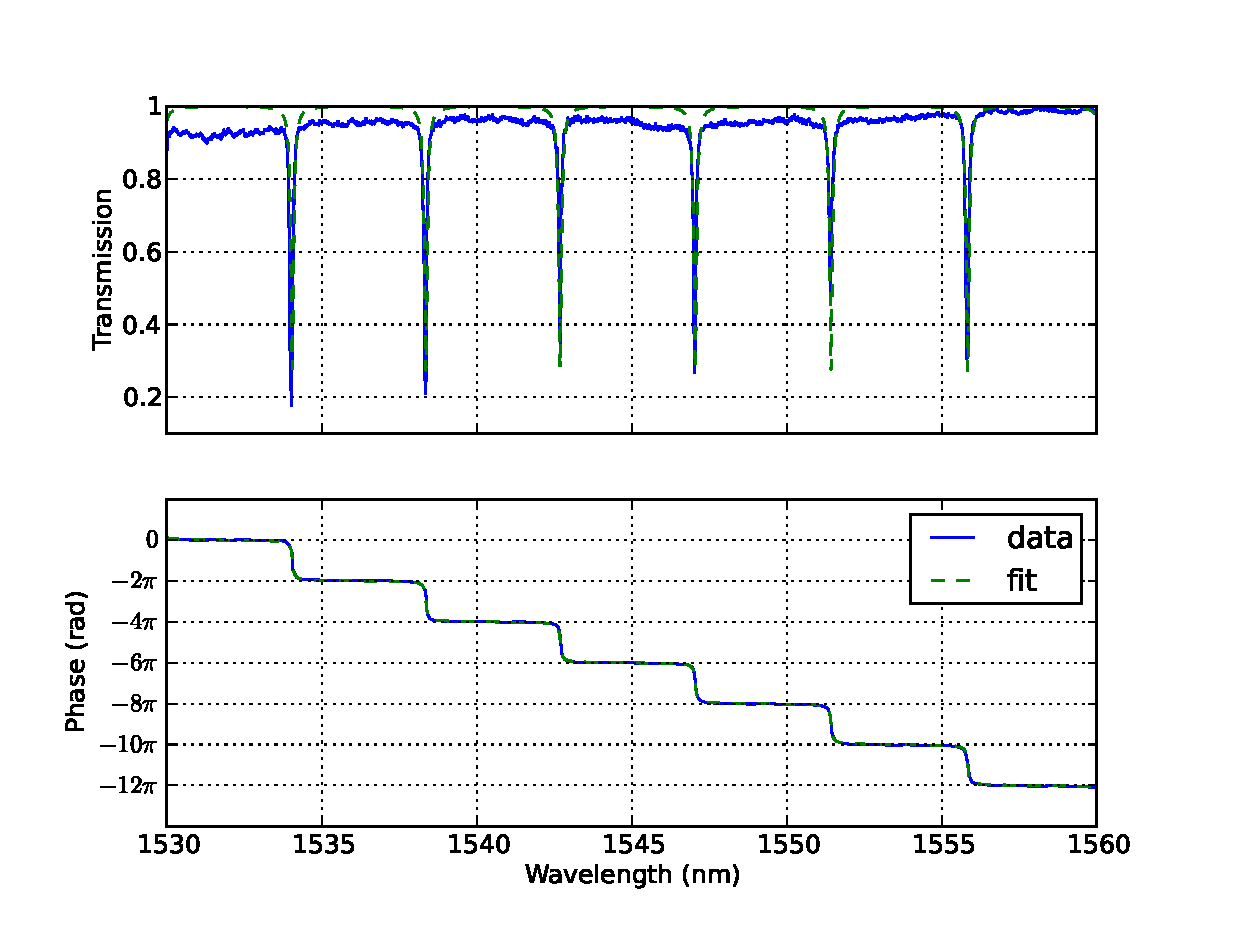
\includegraphics[width=9cm]{r20g200TE_fitPhaseAmp}}
  \centerline{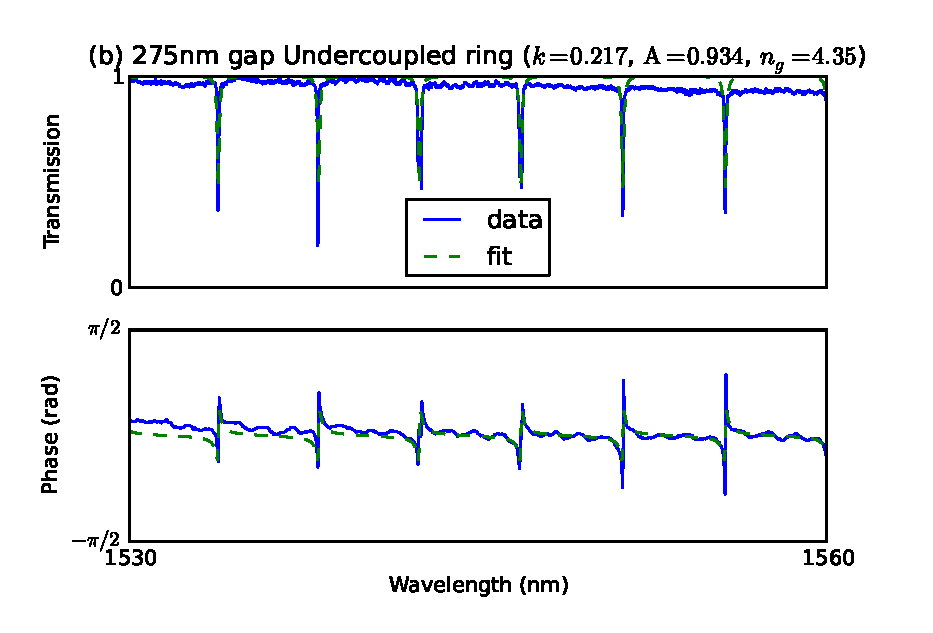
\includegraphics[width=9cm]{r20g275TE_fitPhaseAmp}}
  \caption{We clearly see that over-coupled rings accumulate $2\pi$ phase shifts while under-coupled rings have phase fluctuations in each resonance. }
  \label{fig:overcoupled} % [k = 0.35048909  0.96328564  4.35909895] -25.8545799362 dB/cm 
\end{figure}

% Measurements agree with fits, from which we extract the parameters of the rings.

\subsection{Slow light corrugated waveguides group index}
\label{sec:corrWaveguides}
Traditional group index measurements are based on fringe separation ~\cite{shang81,vlasov:05,yao:811,Dulkeith2006} and path balancing~\cite{Cohen:82,Knox:88,Liang:98} of a Mach-Zehnder interferometer.
In Fig.~\ref{fig:groupIndex} we show the fringes of an interferometer with a 450~$\mu$m corrugated waveguide in one branch and a reference photonic wire on the other branch.
From the wavelength fringe separation ($ \lambda_{min} - \lambda_{max} $) we obtain the variation of the group index with respect to the photonic wire $ n_{g,ref} $~\cite{vlasov:05}:


\begin{equation}
  n_g (\lambda)=\frac{\lambda_{min} \lambda_{max}}{ 2L (\lambda_{min} - \lambda_{max})} + n_{g,ref}
\end{equation}


where $n_{g,ref}$ is the group index of the reference branch, which in our case was obtained from the free spectral range (FSR) of the ring resonators (Eq.~\ref{eq:FSRanillo}).  % $n_{g,ref}=4.36$


On the other hand, our technique provides a continuous phase characterization from which we can extract group index with high resolution only limited by the laser step size.

 
We subtracted the phase evolutions of a 450~$\mu$m and a 27~$\mu$m corrugated waveguide to obtain the phase evolution of a 423~$\mu$m waveguide without the system response.
To balance the interferometer from the short (27~$\mu$m) to the long waveguide (450~$\mu$m), a 11~ps delay increment was necessary in the optical-delay-line.
This means that an equivalent $L=423~\mu$m-long corrugated waveguide has a group delay $T_g=11$~ps, which corresponds to a group index $n_g(\omega_0)=7.8$ (Eq.~\ref{eq:group_index_pathBalancing}).
With the interferometer balanced, we obtained the group index variations around $n_g(\omega_0)$ from the phase evolution slope: %~(Eq.~\ref{eq:groupIndexEvolution}, Fig.~\ref{fig:groupIndex})

\begin{equation}
  n_g (\omega)=  n_g(\omega_0) + \frac{c}{L} \frac{d\phi}{d\omega}
 \label{eq:groupIndexEvolution}
\end{equation}



\begin{figure}[htb]
  \centering
  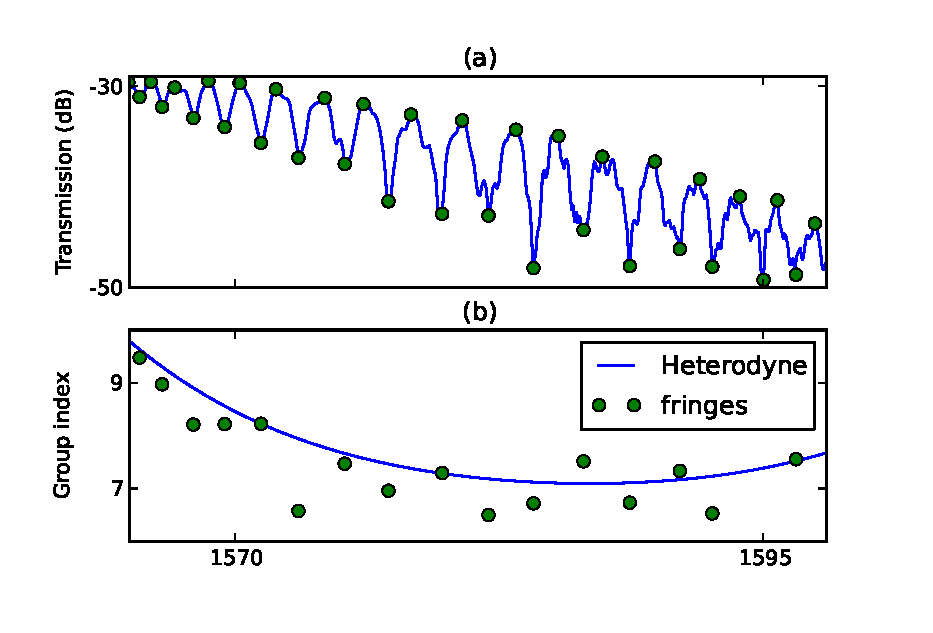
\includegraphics[width=3.5in]{gropIndexComparison_2}
  \caption{Fringes get narrower at the corrugated waveguide band edges, known as slow light regions, where we observe higher group index ($n_g$).
  The proposed continuous measurement (blue dashed line) shows better resolution than traditional fringe-spacing method.}
  \label{fig:groupIndex}
\end{figure}

% In blue dashed line: continuous group index measurement. In green dots, traditional group index measurement using an indirect measurement of the phase with the fringes of a MZI interferometer. Fringes get narrower at the band edges of the corrugated waveguide, known as slow light region, where we observe higher group index ($n_g$).

\section{Conclusion}
We have shown an experimental technique for phase response characterization of integrated photonic components.
The technique cancels out phase noise by using a counter-propagating reference beam, thus avoiding the need of extremely fast tuning rates or cumbersome temperature control schemes.
We characterized a microring resonator and a corrugated waveguide as examples of application.
From the ring resonator phase response, we clearly distinguished overcoupling and undercoupling regimes, observing an excellent agreement with simulations.
In the corrugated waveguide, we measured the group index profile in the slow-light band with better resolution than with a traditional fringe-spacing method.



\section*{Acknowledgments}
We acknowledge financial support from the Spanish Ministry of Science and Innovation through contracts SINADEC (TEC2008- 06333) and PROMETEO/2010/087 NANOFOTONICA. Joaquin Matres is supported by a doctoral grant of the Universidad Polit\'ecnica de Valencia and the Transatlantic partnership for Excellence in Engineering. We also acknowledge Binbin Guan for fruitful discussions and Jose Angel Ayucar and Javier Garcia-Castello help taking the SEM pictures.



% \bibliographystyle{IEEEtran}
% \bibliography{/home/joaquin/Documents/library}

% Generated by IEEEtran.bst, version: 1.13 (2008/09/30)
\begin{thebibliography}{10}
\providecommand{\url}[1]{#1}
\csname url@samestyle\endcsname
\providecommand{\newblock}{\relax}
\providecommand{\bibinfo}[2]{#2}
\providecommand{\BIBentrySTDinterwordspacing}{\spaceskip=0pt\relax}
\providecommand{\BIBentryALTinterwordstretchfactor}{4}
\providecommand{\BIBentryALTinterwordspacing}{\spaceskip=\fontdimen2\font plus
\BIBentryALTinterwordstretchfactor\fontdimen3\font minus
  \fontdimen4\font\relax}
\providecommand{\BIBforeignlanguage}[2]{{%
\expandafter\ifx\csname l@#1\endcsname\relax
\typeout{** WARNING: IEEEtran.bst: No hyphenation pattern has been}%
\typeout{** loaded for the language `#1'. Using the pattern for}%
\typeout{** the default language instead.}%
\else
\language=\csname l@#1\endcsname
\fi
#2}}
\providecommand{\BIBdecl}{\relax}
\BIBdecl

\bibitem{Vanwiggeren2003}
\BIBentryALTinterwordspacing
G.~D. VanWiggeren, A.~R. Motamedi, and D.~M. Barley, ``{Single-scan
  interferometric component analyzer},'' \emph{Photonics Technology Letters,
  IEEE}, vol.~15, no.~2, pp. 263--265, 2003. [Online]. Available:
  \url{http://ieeexplore.ieee.org/xpls/abs\_all.jsp?arnumber=1174140}
\BIBentrySTDinterwordspacing

\bibitem{Gifford2005}
D.~K. Gifford, B.~J. Soller, M.~S. Wolfe, and M.~E. Froggatt, ``{Optical vector
  network analyzer for single-scan measurements of loss, group delay, and
  polarization mode dispersion},'' \emph{Applied optics}, vol.~44, no.~34, pp.
  7282--7286, 2005.

\bibitem{Mas2012}
S.~Mas, J.~Matres, J.~Marti, C.~J. Oton, and J.~Mart\'{\i}, ``{Accurate
  chromatic dispersion characterization of photonic integrated circuits},''
  \emph{Photonics Journal, IEEE}, vol.~4, no.~3, pp. 825--831, Jun. 2012.

\bibitem{Brimont2010}
\BIBentryALTinterwordspacing
A.~Brimont, J.~V. Gal\'{a}n, J.~M. Escalante, J.~Mart\'{\i}, and P.~Sanchis,
  ``{Group-index engineering in silicon corrugated waveguides.}'' \emph{Optics
  letters}, vol.~35, no.~16, pp. 2708--10, Aug. 2010. [Online]. Available:
  \url{http://www.ncbi.nlm.nih.gov/pubmed/20717431}
\BIBentrySTDinterwordspacing

\bibitem{Bogaerts:12}
\BIBentryALTinterwordspacing
W.~Bogaerts, P.~{De Heyn}, T.~{Van Vaerenbergh}, K.~{De Vos}, S.~{Kumar
  Selvaraja}, T.~Claes, P.~Dumon, P.~Bienstman, D.~{Van Thourhout}, and
  R.~Baets, ``{Silicon microring resonators},'' \emph{Laser \& Photonics
  Reviews}, vol.~6, no.~1, pp. 47--73, 2012. [Online]. Available:
  \url{http://dx.doi.org/10.1002/lpor.201100017}
\BIBentrySTDinterwordspacing

\bibitem{McKinnon2009}
\BIBentryALTinterwordspacing
W.~R. McKinnon, D.~X. Xu, C.~Storey, E.~Post, a.~Densmore, a.~Del\^{a}ge,
  P.~Waldron, J.~H. Schmid, and S.~Janz, ``{Extracting coupling and loss
  coefficients from a ring resonator.}'' \emph{Optics express}, vol.~17,
  no.~21, pp. 18\,971--82, Oct. 2009. [Online]. Available:
  \url{http://www.ncbi.nlm.nih.gov/pubmed/20372631}
\BIBentrySTDinterwordspacing

\bibitem{shang81}
H.-T. Shang, ``{Chromatic dispersion measurement by white-light interferometry
  on metre-length single-mode optical fibres},'' \emph{Electronics Letters},
  vol.~17, no.~17, pp. 603--605, 1981.

\bibitem{vlasov:05}
Y.~A. Vlasov, M.~O'Boyle, H.~F. Hamann, and S.~J. McNab, ``{Active control of
  slow light on a chip with photonic crystal waveguides},'' \emph{Nature}, vol.
  438, no. 7064, pp. 65--69, 2005.

\bibitem{yao:811}
\BIBentryALTinterwordspacing
X.~S. Yao and J.~Feinberg, ``{Simple in-line method to measure the dispersion
  of an optical system},'' \emph{Applied Physics Letters}, vol.~62, no.~8, pp.
  811--813, 1993. [Online]. Available:
  \url{http://link.aip.org/link/?APL/62/811/1}
\BIBentrySTDinterwordspacing

\bibitem{Dulkeith2006}
\BIBentryALTinterwordspacing
E.~Dulkeith, F.~Xia, L.~Schares, W.~M.~J. Green, L.~Sekaric, and Y.~A. Vlasov,
  ``{Group index and group velocity dispersion in silicon-on-insulator photonic
  wires.}'' \emph{Optics express}, vol.~14, no.~13, p. 6372, Jun. 2006.
  [Online]. Available:
  \url{http://www.opticsinfobase.org/abstract.cfm?\&amp;id=89589
  http://www.ncbi.nlm.nih.gov/pubmed/19516814}
\BIBentrySTDinterwordspacing

\bibitem{Cohen:82}
L.~G. Cohen and J.~Stone, ``{Interferometric measurements of minimum dispersion
  spectra in short lengths of single-mode fibre},'' \emph{Electronics Letters},
  vol.~18, no.~13, pp. 564--566, 1982.

\bibitem{Knox:88}
\BIBentryALTinterwordspacing
W.~H. Knox, N.~M. Pearson, K.~D. Li, and C.~A. Hirlimann, ``{Interferometric
  measurements of femtosecond group delay in optical components},'' \emph{Opt.
  Lett.}, vol.~13, no.~7, pp. 574--576, Jul. 1988. [Online]. Available:
  \url{http://ol.osa.org/abstract.cfm?URI=ol-13-7-574}
\BIBentrySTDinterwordspacing

\bibitem{Liang:98}
\BIBentryALTinterwordspacing
Y.~Liang and C.~P. Grover, ``{Modified white-light Mach-Zehnder interferometer
  for direct group-delay measurements},'' \emph{Appl. Opt.}, vol.~37, no.~19,
  pp. 4105--4111, Jul. 1998. [Online]. Available:
  \url{http://ao.osa.org/abstract.cfm?URI=ao-37-19-4105}
\BIBentrySTDinterwordspacing

\end{thebibliography}

\end{document}

